\documentclass[tikz,border=10pt]{standalone}
\usepackage{amsmath}
\usetikzlibrary{arrows.meta,decorations.pathmorphing}
\definecolor{ink}{HTML}{21352F}
\definecolor{teal}{HTML}{087F7B}
\definecolor{blue}{HTML}{4B77A8}
\definecolor{gold}{HTML}{C58B2A}

\begin{document}
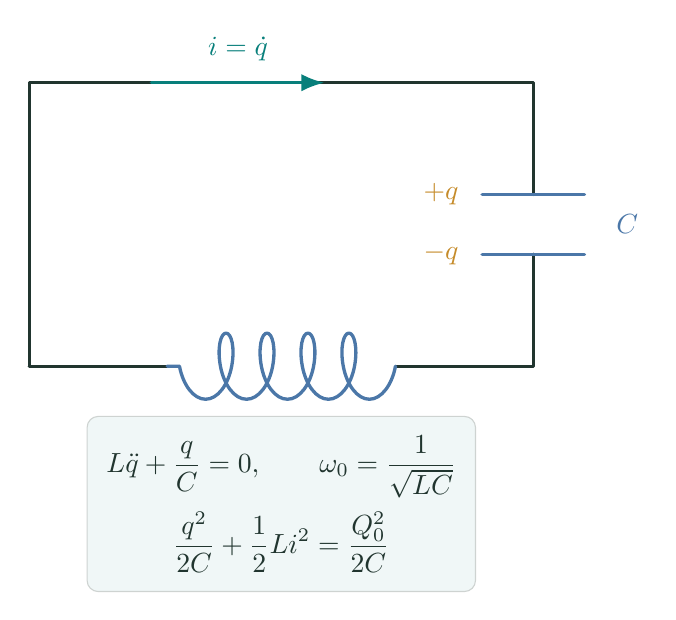
\begin{tikzpicture}[font=\sffamily,text=ink,>=Latex,line cap=round,line join=round]
  % Ideal closed LC loop.
  \draw[ink,very thick] (-3.2,-1.8)--(-3.2,1.8)--(3.2,1.8)--(3.2,.38);
  \draw[ink,very thick] (3.2,-.38)--(3.2,-1.8)--(1.45,-1.8);
  \draw[ink,very thick] (-1.45,-1.8)--(-3.2,-1.8);

  % Capacitor plates.
  \draw[blue,very thick] (2.55,.38)--(3.85,.38);
  \draw[blue,very thick] (2.55,-.38)--(3.85,-.38);
  \node[blue,right=8pt] at (3.85,0) {$C$};
  \node[gold,left=5pt] at (2.55,.38) {$+q$};
  \node[gold,left=5pt] at (2.55,-.38) {$-q$};

  % Inductor.
  \draw[blue,very thick,decorate,
        decoration={coil,aspect=.48,segment length=5.2mm,amplitude=4.2mm}]
    (1.45,-1.8)--(-1.45,-1.8);
  \node[blue,below=8pt] at (0,-2.18) {inductor $L$};

  \draw[teal,very thick,->] (-1.65,1.8)--(.55,1.8)
    node[midway,above=4pt] {$i=\dot q$};

  \node[draw=ink!22,rounded corners=4pt,fill=teal!6,align=center,
        inner sep=7pt] at (0,-3.55)
    {$\displaystyle L\ddot q+\frac qC=0,\qquad
      \omega_0=\frac1{\sqrt{LC}}$\\[4pt]
     $\displaystyle \frac{q^2}{2C}+\frac12Li^2
      =\frac{Q_0^2}{2C}$};
\end{tikzpicture}
\end{document}
